\begin{floatingfigure}{0.3\textwidth}
  \centering
  \tikzstyle{vertex}=[]
  \tikzstyle{arrow}=[thick, -latex]

  \begin{subfigure}[b]{0.3\textwidth}
    \centering
    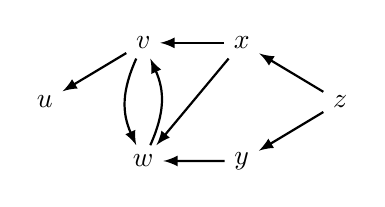
\begin{tikzpicture}[xscale=1.25, yscale=0.75]
      \node[vertex] (u) at (0, 0) {$u$};
      \node[vertex] (v) at (1, 1) {$v$};
      \node[vertex] (w) at (1, -1) {$w$};
      \node[vertex] (x) at (2, 1) {$x$};
      \node[vertex] (y) at (2, -1) {$y$};
      \node[vertex] (z) at (3, 0) {$z$};

      \draw[arrow] (v) to (u);
      \draw[arrow, bend right=15] (v) to (w);
      \draw[arrow, bend right=15] (w) to (v);
      \draw[arrow] (x) to (v);
      \draw[arrow] (x) to (w);
      \draw[arrow] (y) to (w);
      \draw[arrow] (z) to (x);
      \draw[arrow] (z) to (y);
    \end{tikzpicture}
    \caption{A conflict graph}\figlabel{ExamplePreCondensation}
  \end{subfigure}

  \begin{subfigure}[b]{0.3\textwidth}
    \centering
    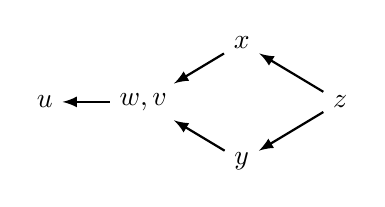
\begin{tikzpicture}[xscale=1.25, yscale=0.75]
      \node[vertex] (u) at (0, 0) {$u$};
      \node[vertex] (vw) at (1, 0) {$w,v$};
      \node[vertex] (x) at (2, 1) {$x$};
      \node[vertex] (y) at (2, -1) {$y$};
      \node[vertex] (z) at (3, 0) {$z$};

      \draw[arrow] (vw) to (u);
      \draw[arrow] (x) to (vw);
      \draw[arrow] (y) to (vw);
      \draw[arrow] (z) to (x);
      \draw[arrow] (z) to (y);
    \end{tikzpicture}
    \caption{The condensed conflict graph}\figlabel{ExampleCondensation}
  \end{subfigure}

  \caption{A conflict graph.}\figlabel{ExampleConflictGraph}
\end{floatingfigure}
